\chapter{Stolen Credentials Problem}
ICN authentication model is based on credentials. A unit with access to credentials can publish authenticated data, and the rest of the network has no way to verify the content authentication other than checking signature validity (created with credentials). Credentials can be loosely categorized into: cold/offline and hot/online. Cold/offline credentials, e.g., private keys, have very long (days or months) or indefinite expiration time; they are typically stored on hard drives and rarely leave the device. Hot/online credentials, e.g., access tokens, are created for a limited period (minutes or hours) and are often transmitted over a communication network. 
Stolen credentials is a serious problem that multi-factor authentication methods try to mitigate, but in this thesis we assume that even such methods cannot solve.
In conjunction with ICN caching, the problem can lead to destructive consequences, because ICN protocols do not provide data revoking/removal functions. A malicious publisher that gains access to stolen credentials can publish authenticated data that can stay in a node's cache for a long time. 

For cold/offline data breaches, we can find reports (DBIR - Data Breach Investigations Report 2020 \cite{2020Data0:online}) showing that 45\% of the attacks are caused by hacking, 22\% by misconfiguration, 22\% by phishing.  17\% caused by malicious software, 4\% by misuse by authorized users, and 4\% by physical interaction.

Most of the attacks (70\%) are performed by external entities motivated financially (86\%). Also, most attacks are targeted at big corporations (72\%). In most of them (58\%), the data breach includes users' personal information.  

From the historical data in Fig. \ref{fig:data-breach-historical} it follows that
\begin{figure}[h!]
    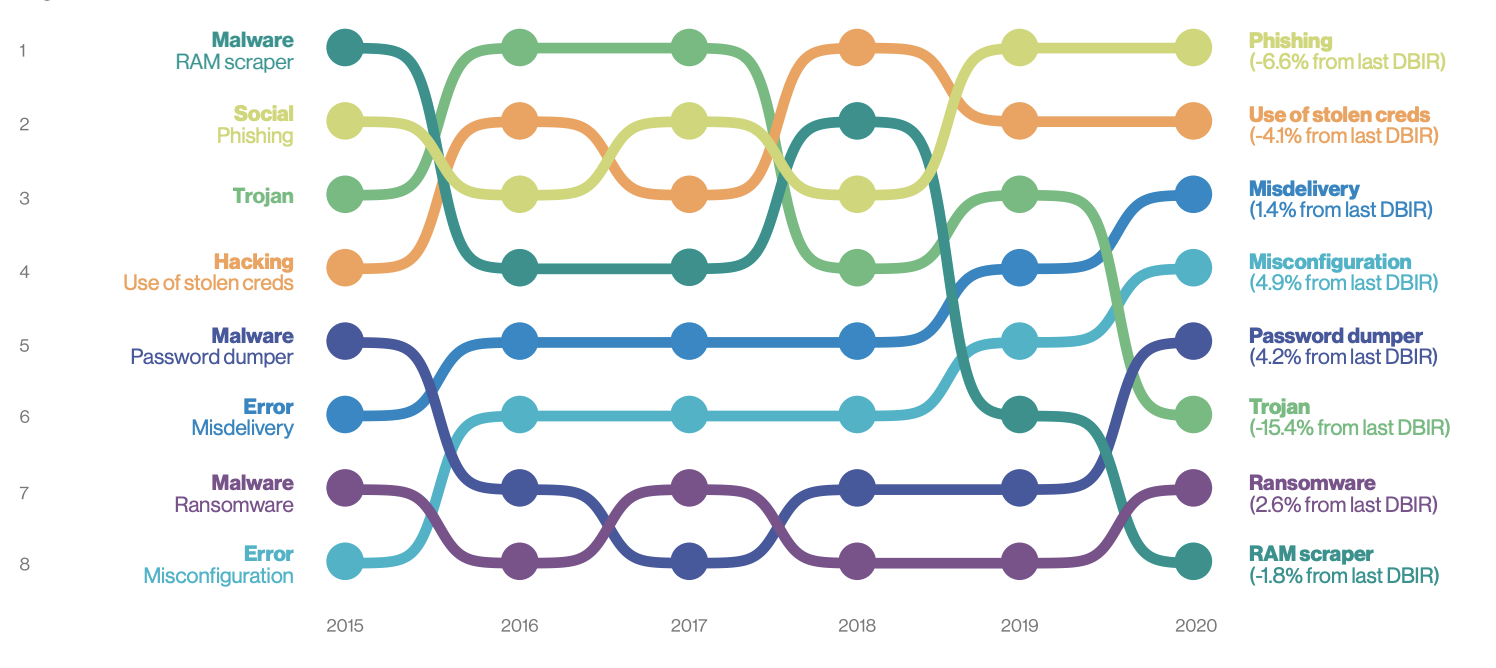
\includegraphics[width=1\textwidth]{img/data-breach-historical.png}
    \centering
    \caption{Change of breaches over time. Source: Data Breach Investigations Report 2020 \cite{2020Data0:online}}
    \label{fig:data-breach-historical}
\end{figure} 
the most visible drop occurs for Trojan horses––from 50\% in 2016 to 5.6\% in 2020. A similar drop occurs for RAM Scrapers, which search the operating system memory for potential confidential data. 
On the contrary, the highest rise can be noted for misconfiguration and accidental data leakage. Yet the highest popularity is still observed for phishing attacks and usage of stolen credentials. 
In Fig. \ref{fig:credentials-steal-discovery}, one sees that for 60\% of the incidents, \textit{the breach was discovered in less than one day}, and this trend is increasing––more incidents are discovered in less than one day. 25\% of incidents were discovered in one or more months. However, it must be noted that some breaches might not have been discovered yet, so the value may be underestimated. In this same report we can find that the number of discoveries has increased due to Managed Security Service Providers (MSSP), which are obligated to publish such breach incidents.

\begin{figure}[h!]
    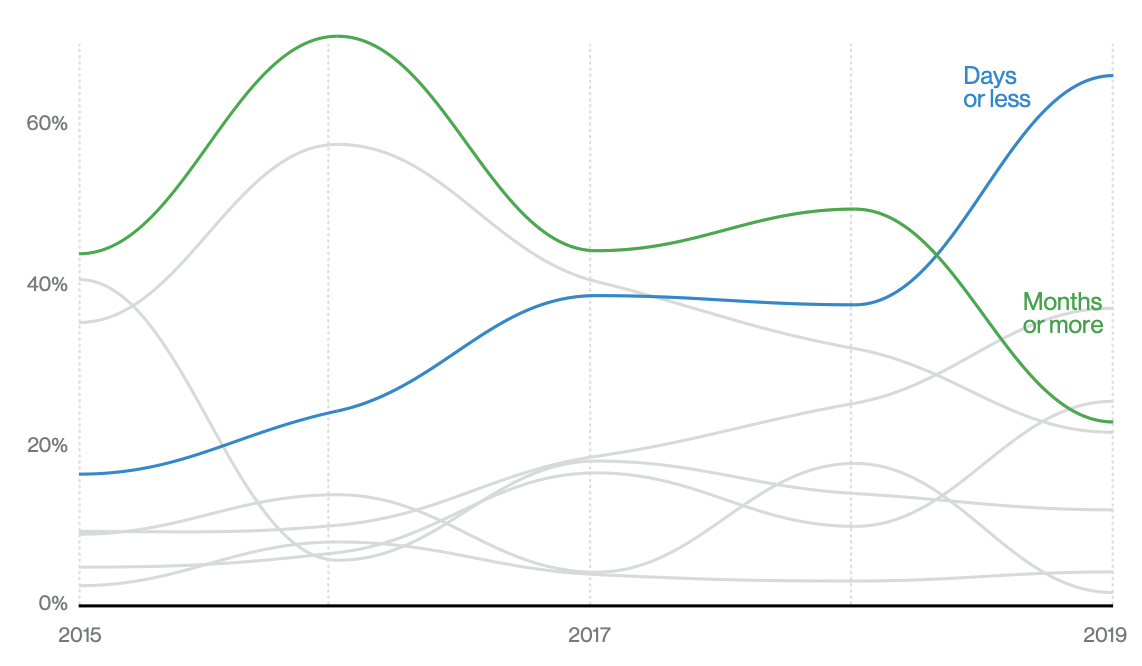
\includegraphics[width=\textwidth]{img/credentials-steal-discovery.png}
    \centering
    \caption{Discovery over time in data breaches. Source: Data Breach Investigations Report 2020 \cite{2020Data0:online}}
    \label{fig:credentials-steal-discovery}
\end{figure} 

Credentials such as access tokens (e.g., JWT tokens) used in communication between two parties have some lifetime duration, after which they expire. In the IETF RFC 6819 document \cite{RFC6819O36:online}, we can find that the suggested lifetime for such credentials ranges from minutes to hours depending on the risk associated with token leakage.